\chapter{Regimes de Volatilidade e o Prêmio de Risco de Volatilidade do Bitcoin}
\label{chap:regimes}

\section{Motivação e Objetivo do Capítulo}
\label{sec:cap9_motivacao}

Os capítulos anteriores estabeleceram que o Prêmio de Risco de Volatilidade do Bitcoin
(BVRP) é positivo em média, contém informação sobre retornos futuros e pode ser utilizado
como sinal em estratégias condicionais. Contudo, os resultados empíricos sugerem
heterogeneidade importante: a relação entre o BVRP e os retornos futuros não é constante
ao longo do tempo, e sua magnitude depende do ambiente de volatilidade vigente.

O indicador de regime de volatilidade realizada figurou como o preditor de maior
importância no modelo de \textit{Random Forest} do Capítulo~\ref{chap:ml_bvrp},
respondendo por aproximadamente 69\% da importância total. Isso motiva a investigação
direta da dependência entre o nível do BVRP, a formação de regimes de volatilidade e
a capacidade preditiva do prêmio sobre os retornos futuros do Bitcoin.

O objetivo deste capítulo é analisar o comportamento do BVRP em diferentes ambientes
de volatilidade. Especificamente, busca-se: (i) caracterizar estatisticamente os
regimes de volatilidade realizada; (ii) testar se a distribuição do BVRP difere
significativamente entre regimes; (iii) avaliar se retornos futuros são estatisticamente
diferentes entre regimes de alta e baixa volatilidade; e (iv) investigar se a
interação entre BVRP e regime de volatilidade tem poder preditivo incremental sobre
os retornos futuros.

\section{Definição dos Regimes de Volatilidade}
\label{sec:cap9_regimes}

Os regimes de volatilidade são definidos com base nos quantis da volatilidade realizada
de 30 dias ($\text{RV}_{30d}$), calculada como desvio-padrão anualizado dos retornos
logarítmicos diários do Bitcoin em janelas móveis de 30 dias. A amostra cobre o período
de 22 de abril de 2021 a 2 de abril de 2026, totalizando 1.776 observações após
o tratamento de dados ausentes.

A classificação é feita por três categorias mutuamente exclusivas:

\begin{itemize}
    \item \textbf{Baixa volatilidade}: $\text{RV}_{30d} \leq q_{25} = 38{,}8\%$;
    \item \textbf{Média volatilidade}: $38{,}8\% < \text{RV}_{30d} < 65{,}9\%$;
    \item \textbf{Alta volatilidade}: $\text{RV}_{30d} \geq q_{75} = 65{,}9\%$.
\end{itemize}

A Tabela~\ref{tab:cap9_frequencia_regimes} apresenta a distribuição das observações
entre os regimes.

\begin{table}[H]
\centering
\small
\caption{Distribuição dos regimes de volatilidade com base nos quantis da RV 30 dias.}
\label{tab:cap9_frequencia_regimes}
\begin{tabular}{lrr}
\toprule
Regime & Observações & Participação (\%) \\
\midrule
Baixa volatilidade & 444 & 25,0\% \\
Média volatilidade & 888 & 50,0\% \\
Alta volatilidade & 444 & 25,0\% \\
\midrule
Total & 1776 & 100,0\% \\
\bottomrule
\end{tabular}
\par\smallskip
\footnotesize\textit{Nota}: Regime de baixa volatilidade: RV 30d $\leq$ 38,8\%; alta volatilidade: RV 30d $\geq$ 65,9\%. Período: 22/04/2021 a 02/04/2026.
\end{table}

Por construção, os regimes extremos concentram 25\% das observações cada, e o regime
intermediário reúne os 50\% centrais da distribuição da RV. A Figura~\ref{fig:cap9_rv30d_regimes}
exibe a série temporal da RV 30 dias com os limiares de regime sobrepostos. Observa-se
que os episódios de alta volatilidade tendem a ocorrer em clusters, refletindo a
persistência temporal da volatilidade (\textit{volatility clustering}) característica
de mercados financeiros e especialmente pronunciada no mercado de criptoativos.

\begin{figure}[H]
\centering
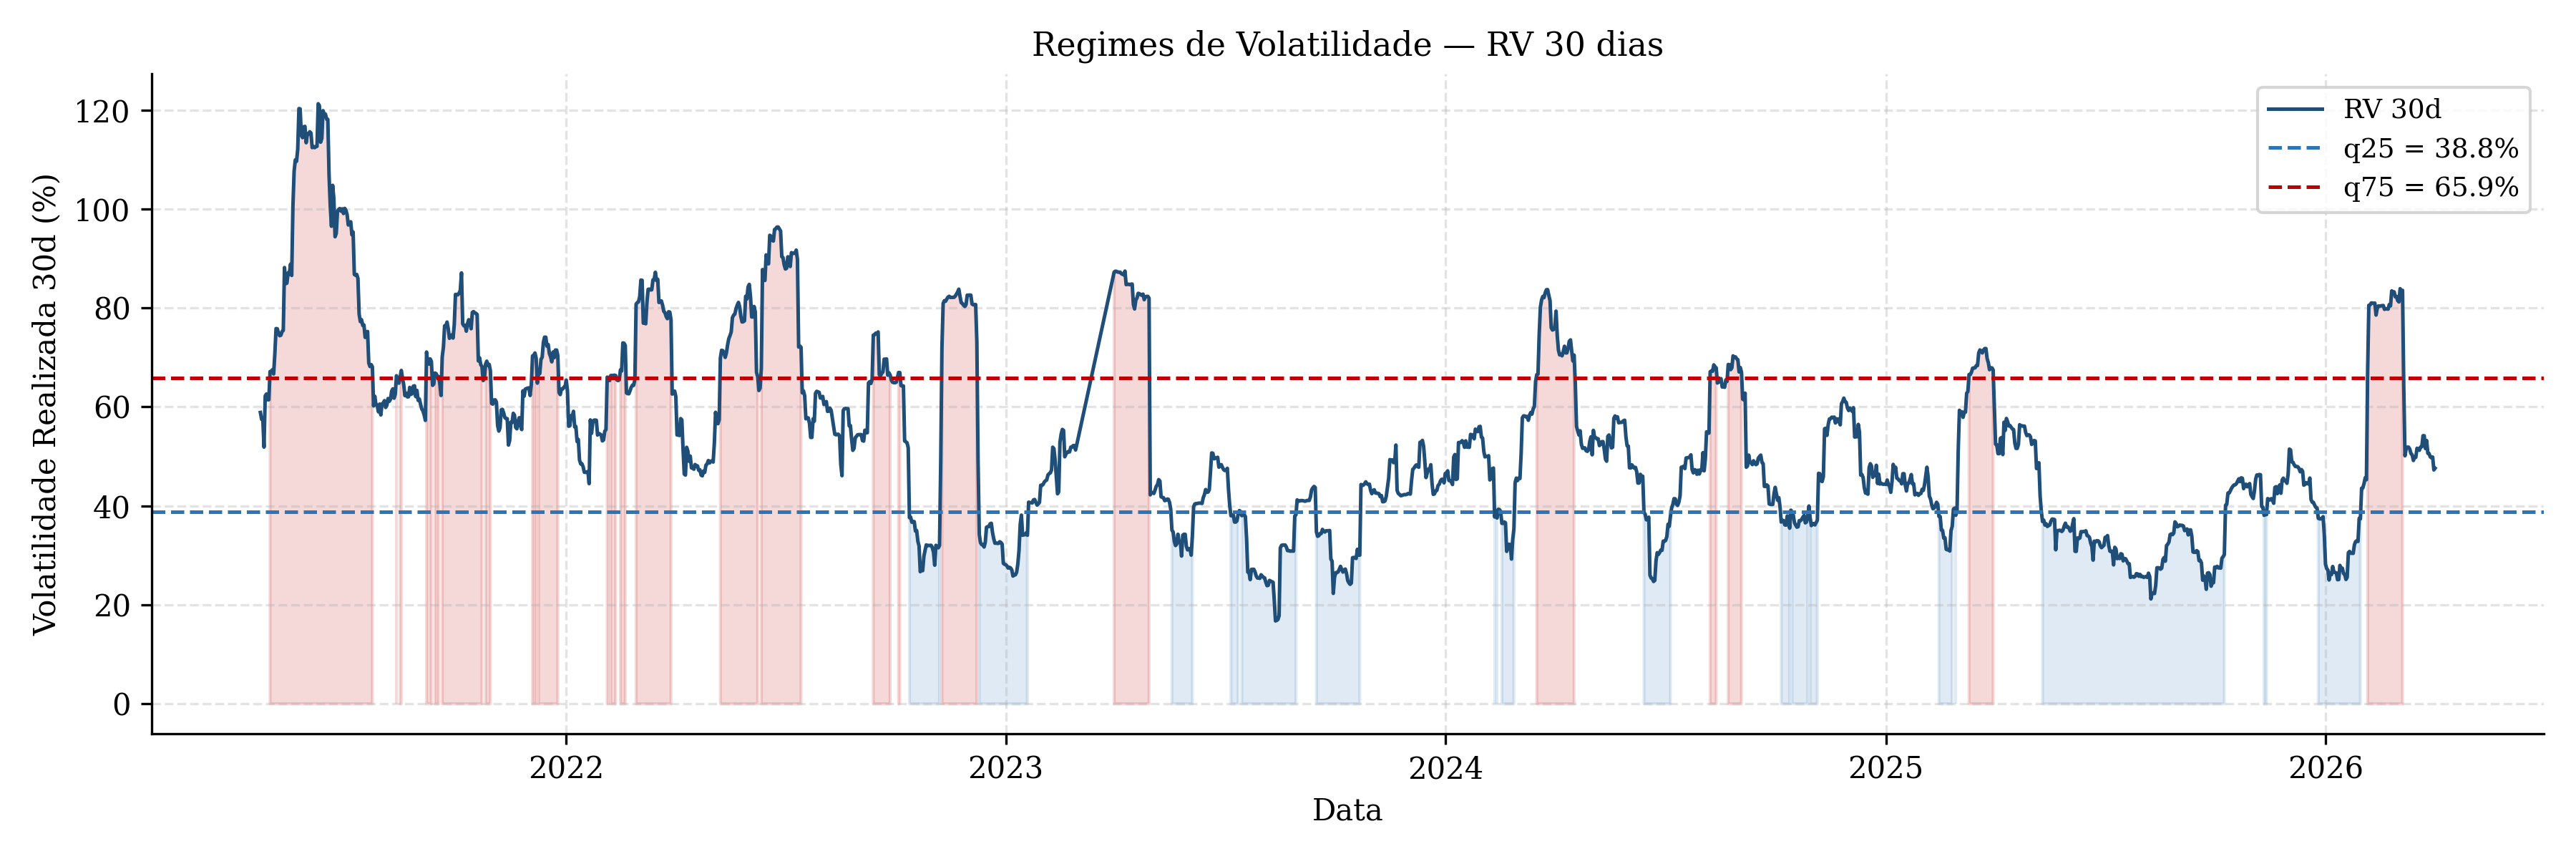
\includegraphics[width=\textwidth]{figs/cap9/fig_cap9_01_rv30d_regimes.png}
\caption{Volatilidade realizada de 30 dias com limiares de regime.
A região azul sombreada indica períodos de baixa volatilidade ($\text{RV}_{30d} \leq 38{,}8\%$);
a região vermelha indica períodos de alta volatilidade ($\text{RV}_{30d} \geq 65{,}9\%$).
Período: 22 abr.\ 2021 -- 2 abr.\ 2026.}
\label{fig:cap9_rv30d_regimes}
\end{figure}

A Figura~\ref{fig:cap9_hist_rv30d} apresenta o histograma da distribuição da RV 30 dias,
mostrando que a distribuição é aproximadamente unimodal com assimetria positiva,
consistente com a literatura de volatilidade em ativos financeiros.

\begin{figure}[H]
\centering
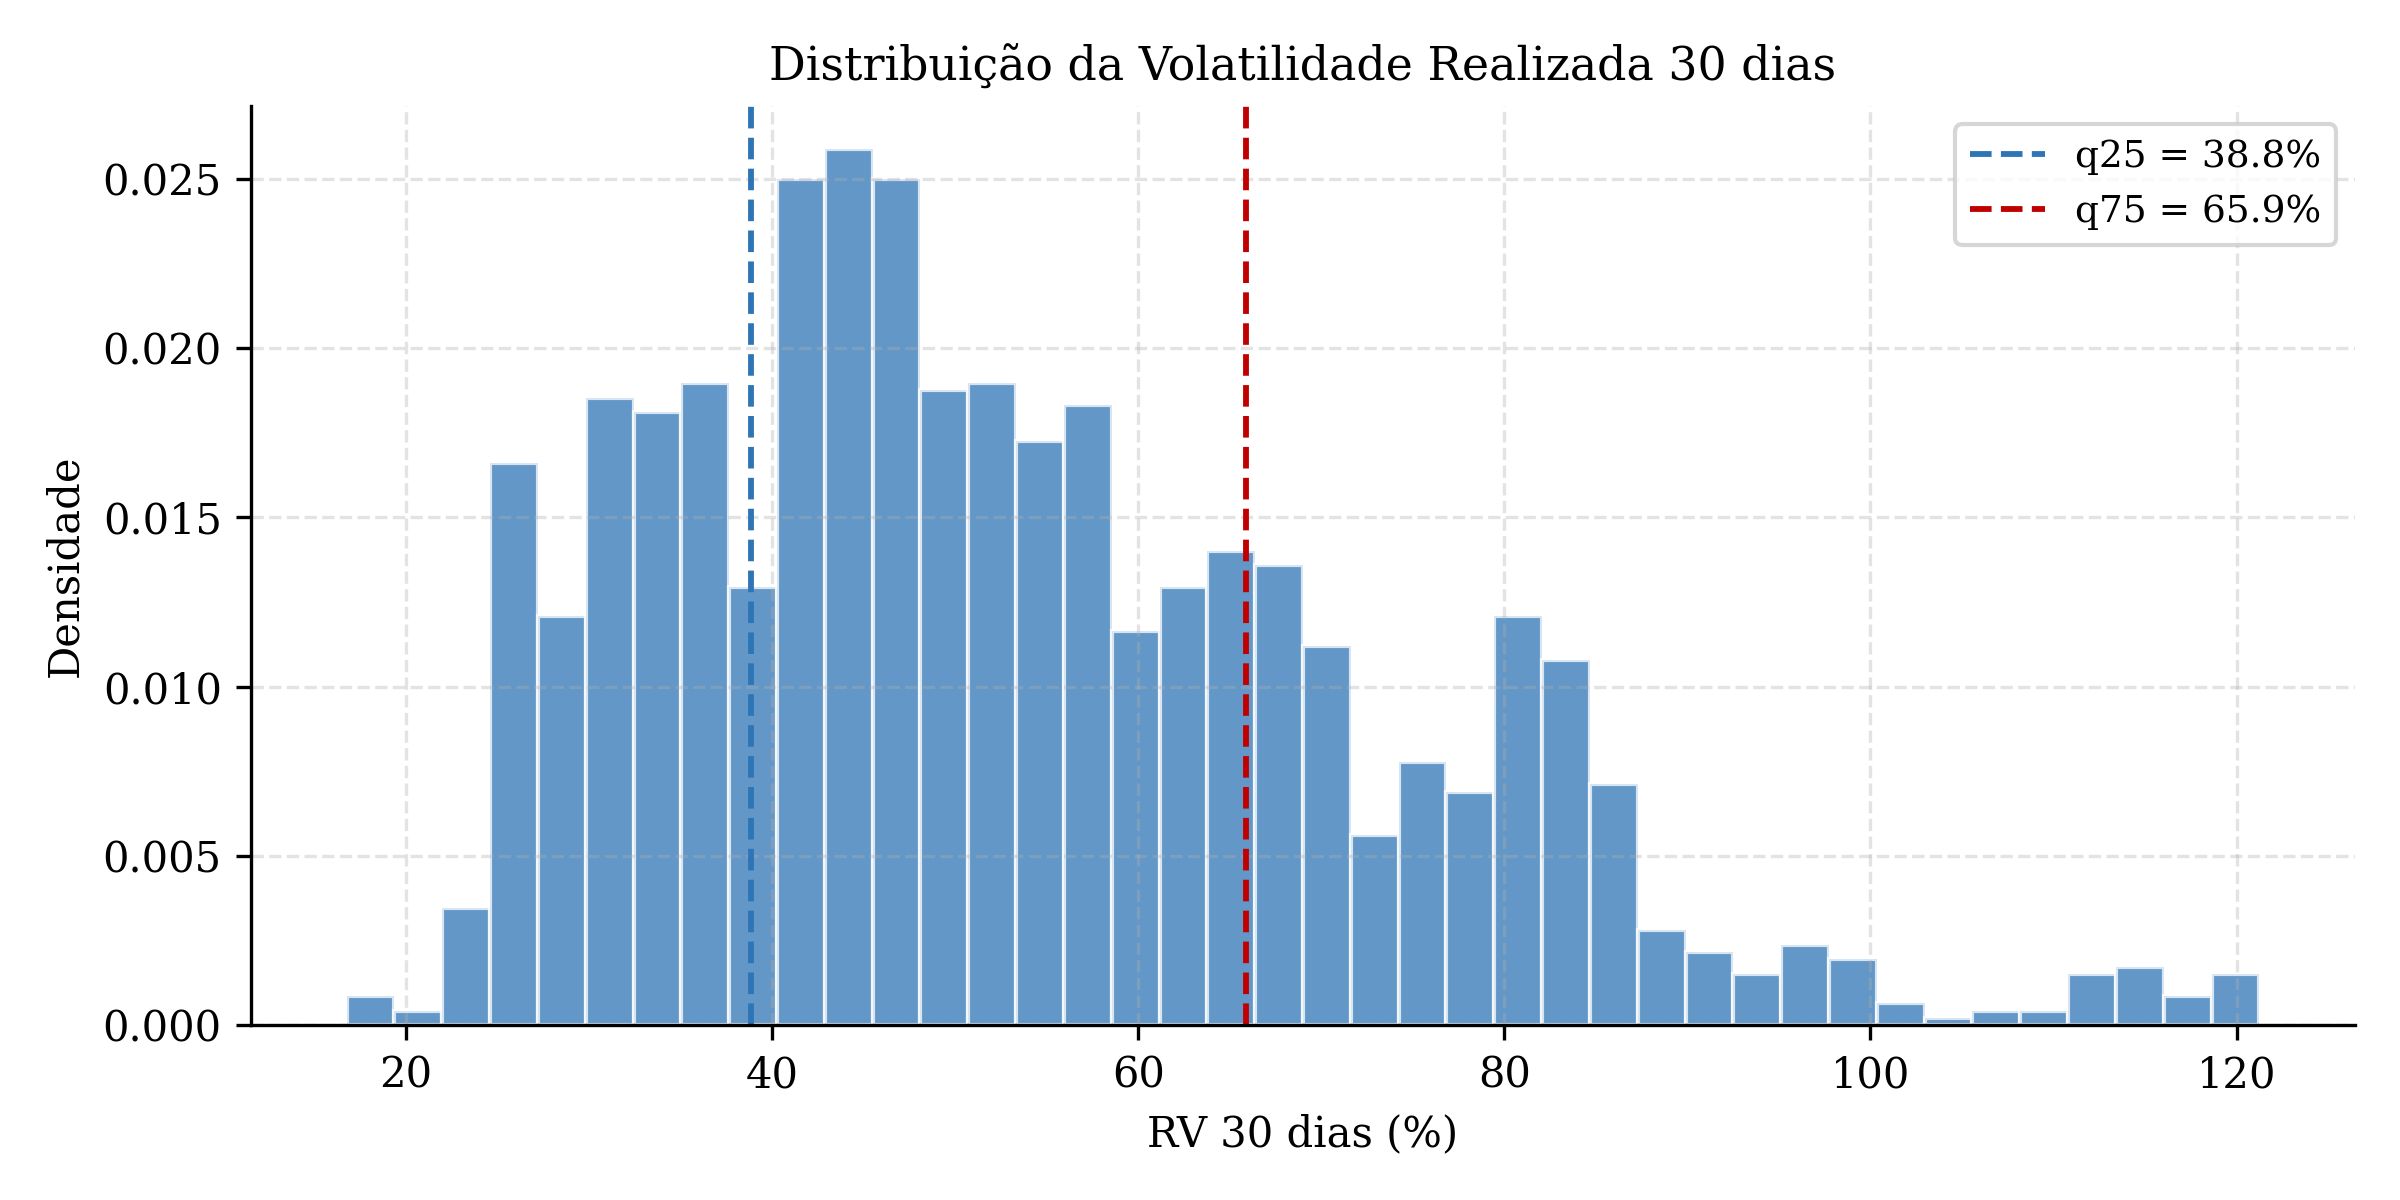
\includegraphics[width=0.75\textwidth]{figs/cap9/fig_cap9_02_hist_rv30d.png}
\caption{Distribuição da volatilidade realizada de 30 dias com limiares de regime.
As linhas tracejadas marcam o primeiro quartil (38,8\%) e o terceiro quartil (65,9\%)
utilizados para definir os regimes.}
\label{fig:cap9_hist_rv30d}
\end{figure}

\section{Caracterização do BVRP por Regime}
\label{sec:cap9_bvrp_regimes}

A Tabela~\ref{tab:cap9_estatisticas_regimes} reporta estatísticas descritivas da
volatilidade realizada (RV 30d), volatilidade implícita (IV 30d) e do BVRP por regime.

\begin{table}[H]
\centering
\small
\caption{Estatísticas descritivas de RV, IV e BVRP por regime de volatilidade.}
\label{tab:cap9_estatisticas_regimes}
\begin{tabular}{llrrrr}
\toprule
Variável & Regime & Média & Mediana & Desvio-padrão & N \\
\midrule
RV 30d & Baixa volatilidade & 31,5320 & 32,0020 & 4,5205 & 444 \\
 & Média volatilidade & 50,9485 & 49,8954 & 7,4026 & 888 \\
 & Alta volatilidade & 80,7655 & 79,7224 & 12,5390 & 444 \\
\midrule
IV 30d & Baixa volatilidade & 44,7845 & 42,1550 & 8,5492 & 444 \\
 & Média volatilidade & 60,9609 & 57,1950 & 13,7285 & 888 \\
 & Alta volatilidade & 79,2680 & 80,7550 & 18,6945 & 444 \\
\midrule
BVRP & Baixa volatilidade & 13,2524 & 11,5445 & 7,5059 & 444 \\
 & Média volatilidade & 10,0124 & 9,0522 & 10,4147 & 888 \\
 & Alta volatilidade & -1,4976 & -0,4144 & 16,4940 & 444 \\
\bottomrule
\end{tabular}
\end{table}

O resultado mais relevante é a inversão do sinal médio do BVRP entre regimes. No regime
de baixa volatilidade, o BVRP médio é de 13,25 p.p., indicando que a volatilidade
implícita supera sistematicamente a realizada --- o mercado paga um prêmio positivo
por proteção mesmo em ambientes calmos. No regime de média volatilidade, o prêmio
permanece positivo e significativo (10,01 p.p.), embora com maior dispersão
(desvio-padrão de 10,41 p.p.).

No regime de alta volatilidade, contudo, o BVRP médio torna-se negativo ($-1{,}50$ p.p.),
com desvio-padrão de 16,49 p.p. Isso indica que, em ambientes de estresse, a volatilidade
realizada frequentemente supera a implícita: os movimentos efetivos do Bitcoin são maiores
do que o mercado de opções precificava antecipadamente. Este resultado é economicamente
coerente com a literatura de \textit{crash risk} em criptoativos: durante episódios de
crise, a volatilidade irrompe de forma não antecipada, comprometendo a capacidade da
IV de servir como seguro eficaz.

A Figura~\ref{fig:cap9_boxplot_bvrp_regimes} ilustra estas diferenças por meio de
diagramas de caixa.

\begin{figure}[H]
\centering
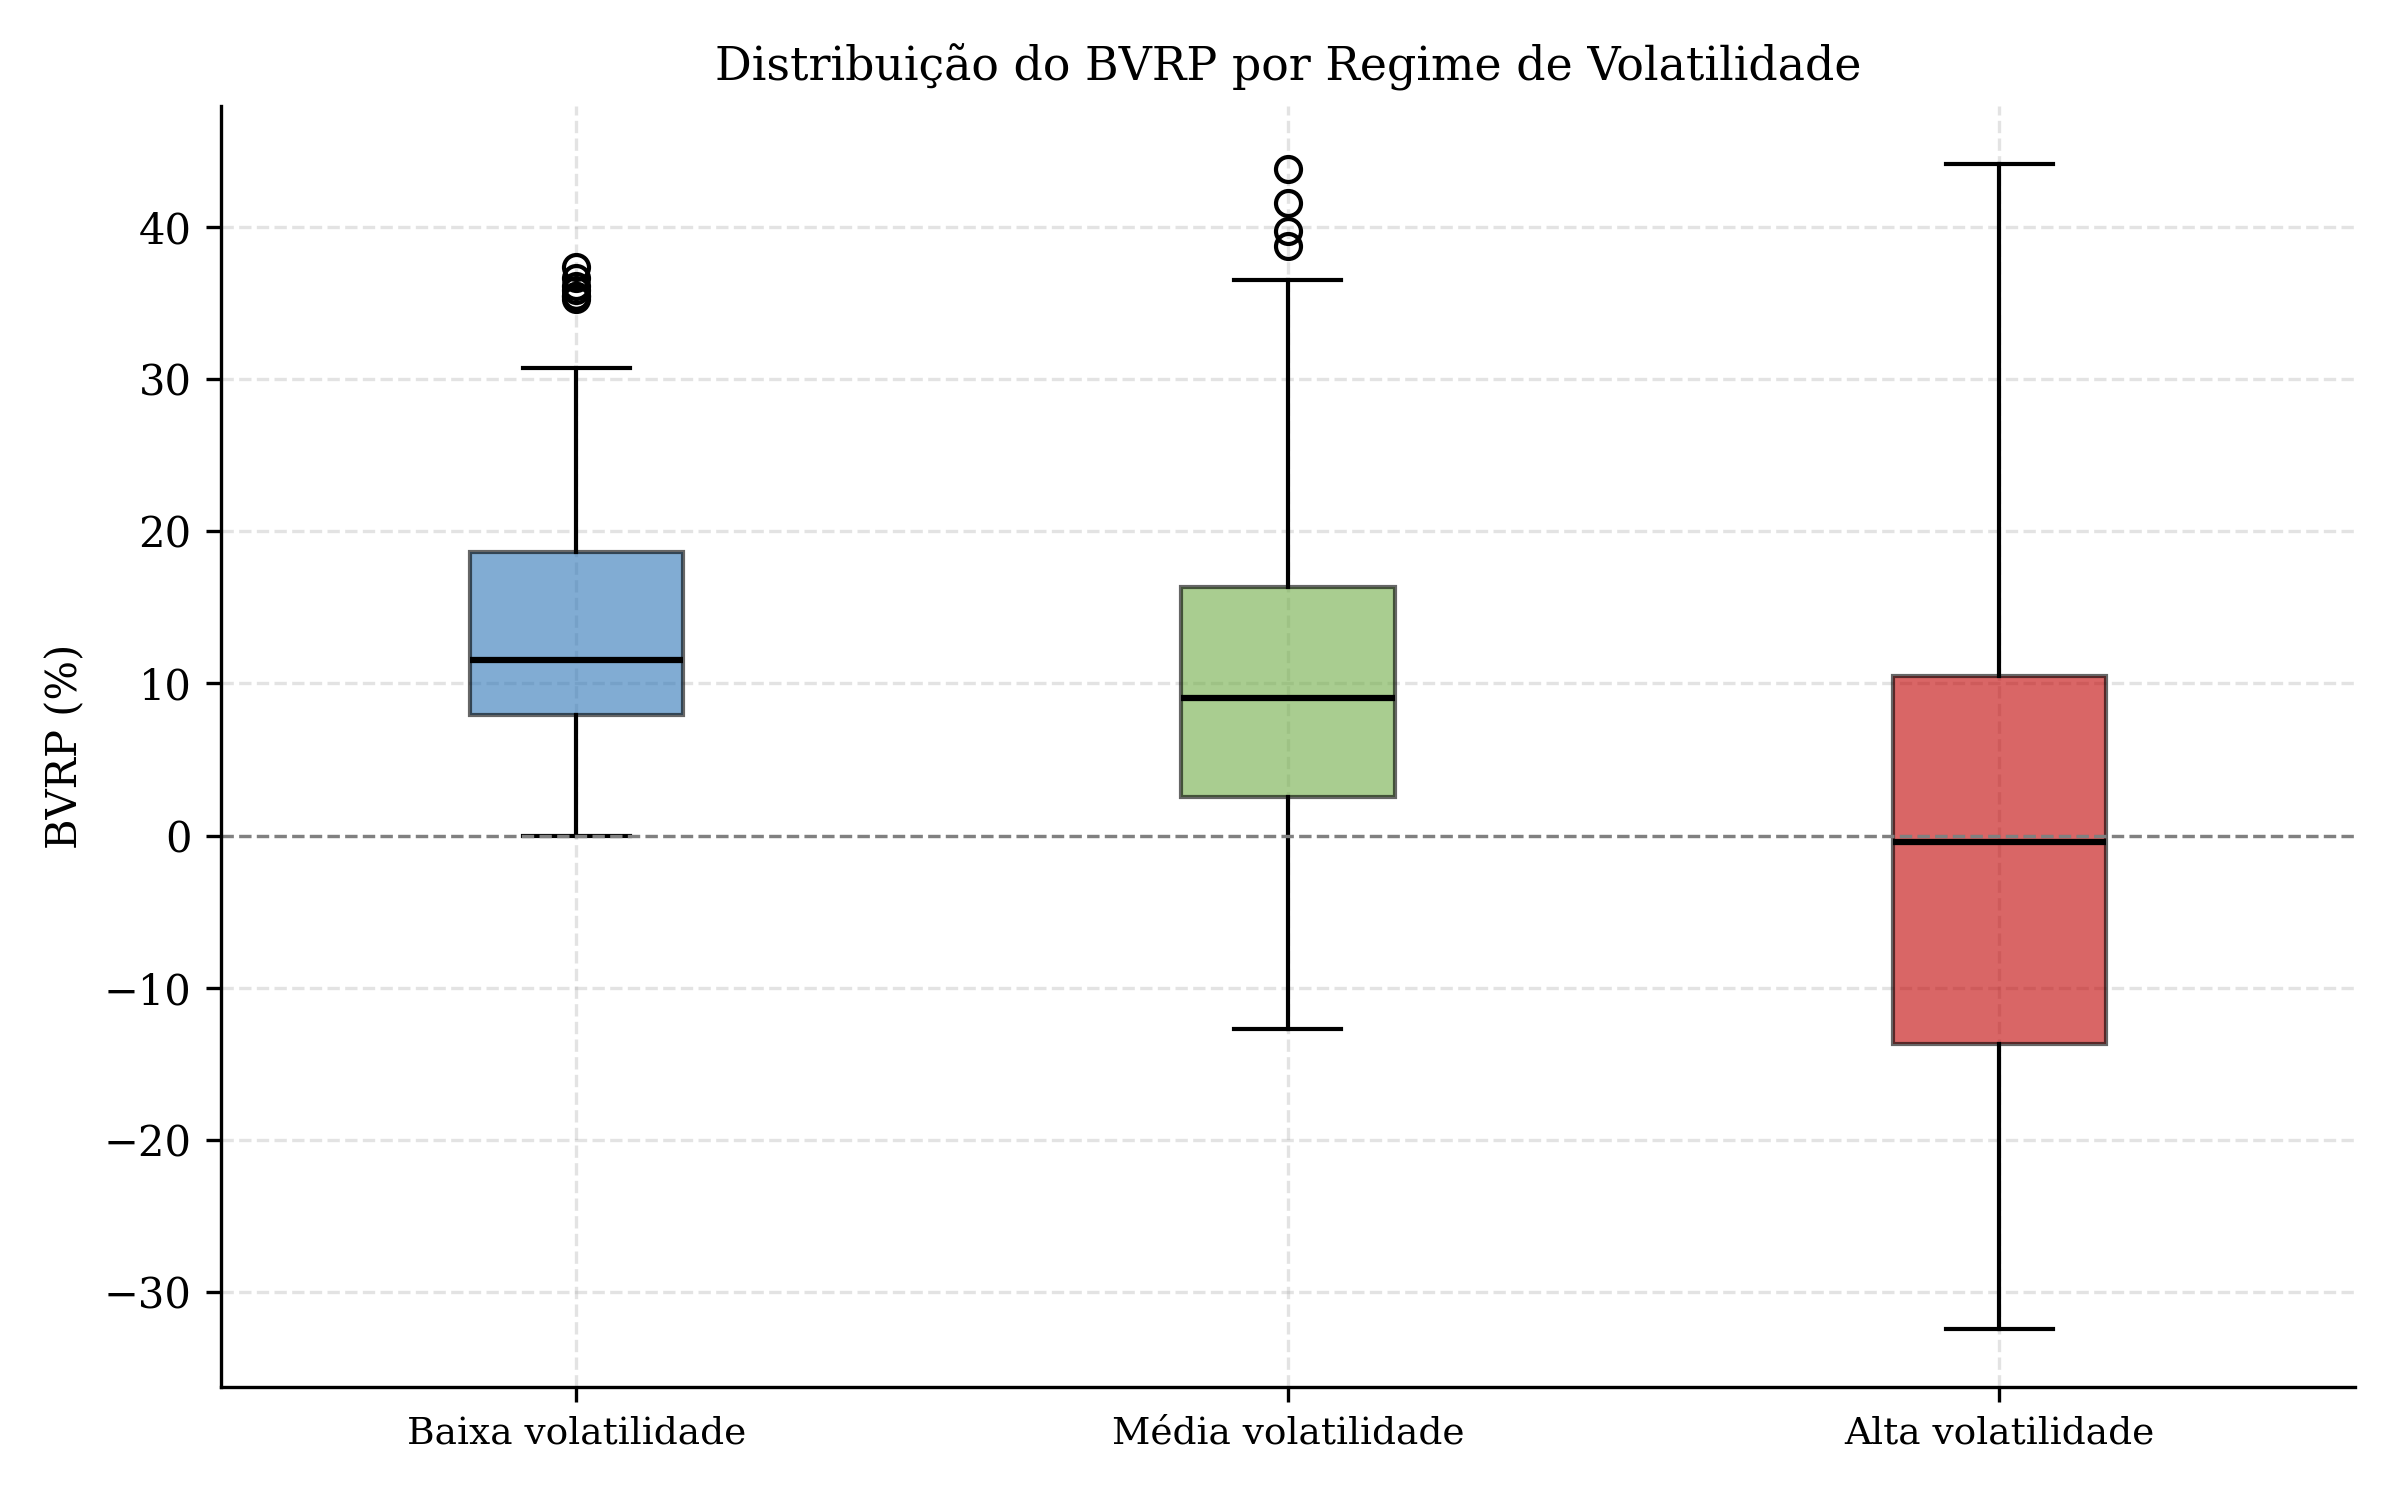
\includegraphics[width=0.72\textwidth]{figs/cap9/fig_cap9_03_boxplot_bvrp_regimes.png}
\caption{Distribuição do BVRP por regime de volatilidade. A linha horizontal tracejada
marca o nível zero. No regime de alta volatilidade, a mediana do BVRP é próxima de zero
($-0{,}41$ p.p.) com distribuição altamente dispersa, enquanto nos regimes de baixa e
média volatilidade o prêmio é consistentemente positivo.}
\label{fig:cap9_boxplot_bvrp_regimes}
\end{figure}

\section{Retornos Futuros por Regime de Volatilidade}
\label{sec:cap9_retornos}

A Tabela~\ref{tab:cap9_retornos_regimes} apresenta o retorno futuro médio do Bitcoin
para cada combinação de regime e horizonte de previsão.

\begin{table}[H]
\centering
\small
\caption{Retorno futuro médio (\%) por regime de volatilidade e horizonte.}
\label{tab:cap9_retornos_regimes}
\begin{tabular}{lrrrrr}
\toprule
Regime & 1d & 5d & 10d & 20d & 30d \\
\midrule
Baixa volatilidade & 0,0717 & 0,4608 & 1,0926 & 2,8820 & 4,8610 \\
Média volatilidade & 0,0769 & 0,3291 & 0,4419 & 0,6473 & 0,9256 \\
Alta volatilidade & 0,0272 & -0,0048 & 0,1743 & 0,3133 & 0,0602 \\
\bottomrule
\end{tabular}
\end{table}

O padrão é monotônico e economicamente relevante: em todos os horizontes avaliados
(1, 5, 10, 20 e 30 dias), o retorno futuro médio é maior no regime de baixa
volatilidade do que no regime de alta. Para horizontes curtos (1 dia), as diferenças
são pequenas e potencialmente ruídosas. Para horizontes mais longos (20 e 30 dias),
a diferença se torna economicamente substancial: no regime de baixa volatilidade,
o retorno médio acumulado em 30 dias é de 3,29\%, ao passo que no regime de alta
volatilidade é de $-1{,}52\%$.

\subsection{Testes de Significância Estatística}
\label{sec:cap9_ttest}

A Tabela~\ref{tab:cap9_ttest} reporta o teste $t$ de Welch comparando as médias dos
retornos futuros entre os regimes de alta e baixa volatilidade.

\begin{table}[H]
\centering
\small
\caption{Teste $t$ de Welch: diferença de retornos futuros entre regimes de alta e baixa volatilidade.}
\label{tab:cap9_ttest}
\begin{tabular}{lrrrrc}
\toprule
Horizonte & Média Alta Vol & Média Baixa Vol & Diferença & $t$-stat & $p$-valor \\
\midrule
1d & -0,1211 & 0,0790 & -0,2000 & -1,0115 & 0,3121 \\
5d & -0,4767 & 0,3466 & -0,8233 & -1,8703 & 0,0618* \\
10d & -0,6771 & 0,7295 & -1,4065 & -2,1138 & 0,0348** \\
20d & -1,1289 & 1,9304 & -3,0593 & -3,1219 & 0,0019*** \\
30d & -1,5224 & 3,2866 & -4,8089 & -4,0770 & 0,0000*** \\
\bottomrule
\end{tabular}
\par\smallskip
\footnotesize\textit{Nota}: Retornos expressos em \%. *** $p<0{,}01$; ** $p<0{,}05$; * $p<0{,}10$.
\end{table}

A diferença entre retornos em regimes de alta e baixa volatilidade é estatisticamente
significativa a partir do horizonte de 10 dias ($p=0{,}0348$), tornando-se
altamente significativa nos horizontes de 20 dias ($p=0{,}0019$) e 30 dias
($p<0{,}0001$). No horizonte de 1 dia, a diferença não é estatisticamente detectável
($p=0{,}312$), consistente com a hipótese de eficiência de mercado de curto prazo.

Estes resultados indicam que o regime de volatilidade realizada contém informação
preditiva sobre retornos futuros do Bitcoin, especialmente em horizontes médios
a longos. Em ambientes de alta volatilidade, os retornos médios subsequentes tendem
a ser negativos, ao passo que em ambientes de baixa volatilidade os retornos médios
são positivos e estatisticamente diferentes de zero para horizontes a partir de 20 dias.

A Figura~\ref{fig:cap9_boxplot_ret_regimes} ilustra as distribuições condicionais
dos retornos futuros para os horizontes de 5, 10 e 20 dias.

\begin{figure}[H]
\centering
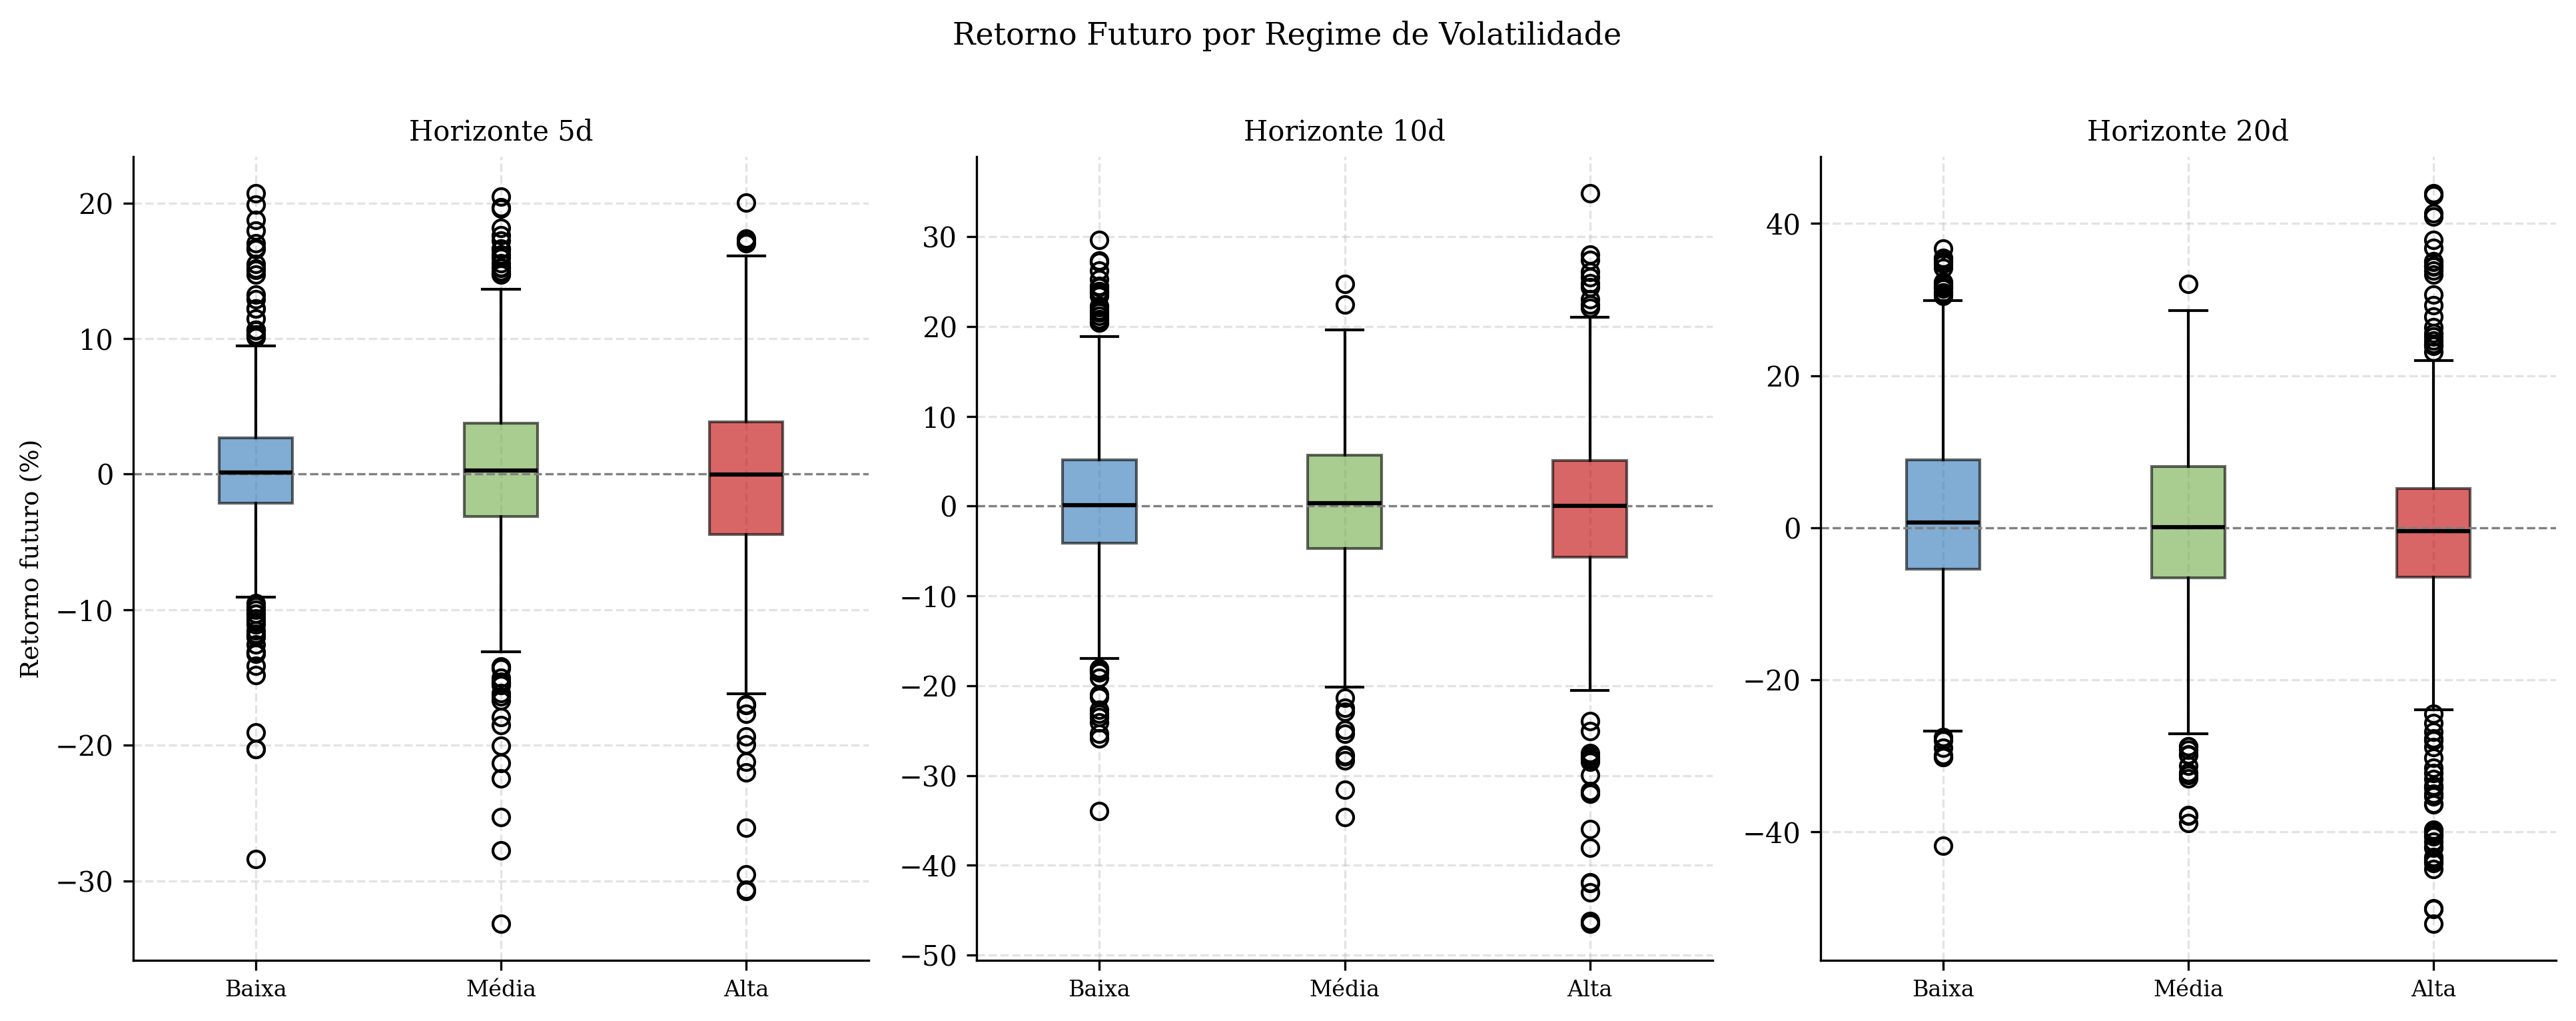
\includegraphics[width=\textwidth]{figs/cap9/fig_cap9_04_boxplot_ret_regimes.png}
\caption{Distribuição dos retornos futuros por regime de volatilidade para horizontes
de 5, 10 e 20 dias. A dispersão aumenta com o horizonte, mas a separação entre as
medianas dos regimes de alta e baixa volatilidade torna-se progressivamente mais
pronunciada.}
\label{fig:cap9_boxplot_ret_regimes}
\end{figure}

\section{Análise de Regressão Condicional}
\label{sec:cap9_regressao}

Para avaliar se a interação entre o BVRP e o regime de volatilidade tem poder preditivo
incremental sobre os retornos futuros, estimam-se regressões condicionais da forma:

\begin{equation}
r_{t+h} = \alpha + \beta_1 \cdot \text{BVRP}_t
          + \beta_2 \cdot D_t^{\text{alto}}
          + \beta_3 \cdot \left(\text{BVRP}_t \times D_t^{\text{alto}}\right) + \varepsilon_{t+h},
\label{eq:cap9_reg_condicional}
\end{equation}

\noindent onde $r_{t+h}$ é o retorno logarítmico acumulado do Bitcoin de $t$ a $t+h$,
$D_t^{\text{alto}}$ é uma variável indicadora igual a 1 quando o Bitcoin se encontra
em regime de alta volatilidade ($\text{RV}_{30d} \geq q_{75}$), e
$\text{BVRP}_t \times D_t^{\text{alto}}$ é o termo de interação entre o prêmio e
o regime. Os erros-padrão são calculados pelo método de Newey--West com $h$
defasagens, para corrigir autocorrelação e heteroscedasticidade induzidas pela
sobreposição das janelas de retorno.

\begin{table}[H]
\centering
\small
\caption{Regressões condicionais do retorno futuro em função do BVRP e do regime de volatilidade.
Erros-padrão de Newey--West com $h$ defasagens. Coeficientes com $t$-estatísticas entre parênteses.}
\label{tab:cap9_regressoes}
\begin{tabular}{lrrrrr}
\toprule
Variável & 1d & 5d & 10d & 20d & 30d \\
\midrule
Constante & 0,0003 & 0,0039 & 0,0091 & 0,0268* & 0,0410* \\
 & (0,2677) & (0,8822) & (1,1470) & (1,6853) & (1,6720) \\
\addlinespace[2pt]
BVRP & 0,0000 & -0,0001 & -0,0004 & -0,0017 & -0,0025 \\
 & (0,3123) & (-0,3375) & (-0,6917) & (-1,3881) & (-1,4091) \\
\addlinespace[2pt]
Alta Volatilidade & -0,0013 & -0,0084 & -0,0154 & -0,0370 & -0,0557 \\
 & (-0,6783) & (-1,0743) & (-1,0089) & (-1,2207) & (-1,2603) \\
\addlinespace[2pt]
BVRP $\times$ Alta Vol & 0,0001 & 0,0003 & 0,0007 & 0,0024 & 0,0029 \\
 & (0,6499) & (0,6178) & (0,8882) & (1,5669) & (1,3769) \\
\addlinespace[2pt]
\midrule
$R^2$ & 0,0019 & 0,0033 & 0,0051 & 0,0171 & 0,0221 \\
$N$ & 1776 & 1776 & 1776 & 1776 & 1776 \\
\bottomrule
\end{tabular}
\par\smallskip
\footnotesize\textit{Nota}: *** $p<0{,}01$; ** $p<0{,}05$; * $p<0{,}10$.
\end{table}

Os resultados da Tabela~\ref{tab:cap9_regressoes} revelam que nenhum dos coeficientes
é estatisticamente significativo a 5\% em nenhum horizonte, com exceção marginal da
constante para os horizontes de 20 e 30 dias (10\% de significância). O $R^2$ das
regressões é baixo em todos os horizontes, variando de 0,19\% (1 dia) a 2,21\% (30 dias),
refletindo a dificuldade estrutural de prever retornos diários de ativos especulativos.

Individualmente, o coeficiente $\hat{\beta}_1$ (BVRP) apresenta sinal negativo em todos
os horizontes a partir de 5 dias, sugerindo que, controlando pelo regime, níveis mais
elevados de BVRP não necessariamente predizem retornos futuros mais altos --- resultado
coerente com a hipótese de que o BVRP elevado em regimes de alta volatilidade reflete
compensação por risco já materializado, e não antecipação de retornos positivos futuros.

O coeficiente $\hat{\beta}_2$ (dummy de alta volatilidade) é negativo em todos os
horizontes, confirmando o padrão identificado no teste $t$: períodos de alta volatilidade
estão associados a retornos futuros menores. O coeficiente $\hat{\beta}_3$ (interação
BVRP $\times$ alta vol) é positivo, sugerindo que, dentro do regime de alta volatilidade,
um BVRP marginalmente mais alto pode atenuar parcialmente o efeito negativo do regime
sobre os retornos; contudo, o coeficiente não é significativo em nenhum horizonte.

A ausência de significância estatística nas regressões individuais não contradiz os
resultados do teste $t$: as regressões condicionais testam efeitos marginais
conjuntos (BVRP e regime de forma simultânea), enquanto o teste $t$ compara
médias incondicionais por regime. A multicolinearidade entre o BVRP e a dummy de
regime --- dado que o prêmio médio é correlacionado com o regime, como demonstrado
na Seção~\ref{sec:cap9_bvrp_regimes} --- pode atenuar a significância individual
dos coeficientes mesmo quando os efeitos de regime são economicamente relevantes.

A Figura~\ref{fig:cap9_scatter_bvrp_ret} apresenta diagramas de dispersão do BVRP
versus retorno futuro, desagregados por regime, para os horizontes de 5, 10 e 20 dias.

\begin{figure}[H]
\centering
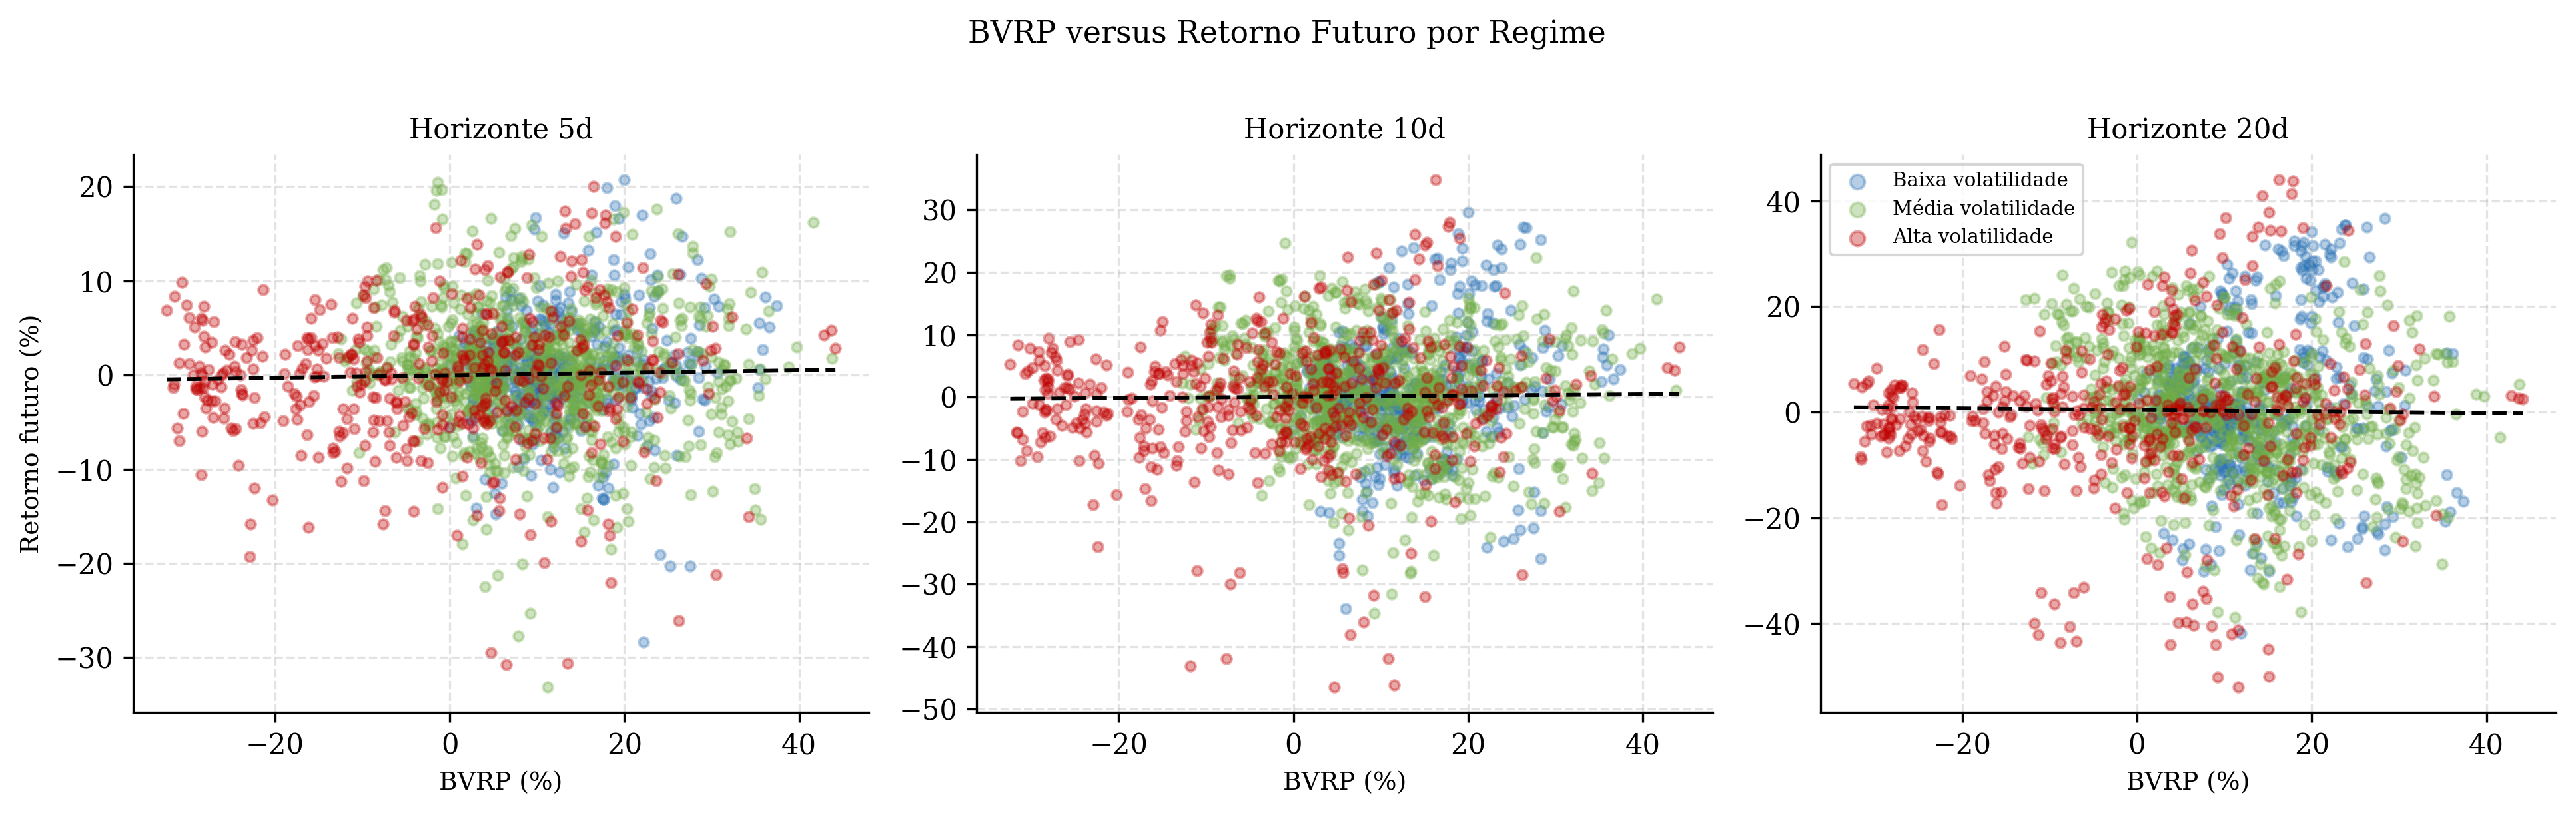
\includegraphics[width=\textwidth]{figs/cap9/fig_cap9_05_scatter_bvrp_ret.png}
\caption{Dispersão do BVRP versus retorno futuro por regime de volatilidade.
A linha tracejada representa a linha de tendência linear incondicional para toda
a amostra. A separação vertical entre os pontos dos regimes de alta (vermelho) e
baixa (azul) volatilidade torna-se progressivamente mais pronunciada com o horizonte,
consistente com os resultados do teste $t$.}
\label{fig:cap9_scatter_bvrp_ret}
\end{figure}

\section{Síntese dos Resultados}
\label{sec:cap9_sintese}

Os resultados deste capítulo revelam três achados centrais sobre a relação entre
regimes de volatilidade e o BVRP no mercado de Bitcoin:

\textbf{1. O BVRP é estruturalmente dependente do regime.}
O prêmio médio é substancialmente maior em regimes de baixa volatilidade (13,25 p.p.)
do que em regimes de alta (−1,50 p.p.). Em ambientes de estresse, a volatilidade
realizada frequentemente supera a implícita, tornando o prêmio negativo e elevando
a incerteza sobre o retorno da estratégia de venda de volatilidade.

\textbf{2. O regime de volatilidade prediz retornos futuros em horizontes médios e longos.}
Retornos futuros são significativamente menores em regimes de alta volatilidade
para horizontes de 10 a 30 dias. A diferença não é detectável estatisticamente no
horizonte de 1 dia, o que é consistente com a eficiência informacional de curto prazo.

\textbf{3. A interação BVRP $\times$ regime não tem poder preditivo incremental robusto.}
As regressões condicionais não identificam um efeito significativo da interação
entre o nível do BVRP e o regime sobre os retornos futuros. O efeito preditivo
do regime opera predominantemente de forma aditiva, e não através de uma modulação
do poder preditivo do BVRP por nível de volatilidade.

Em conjunto, estes resultados são consistentes com a visão de que a estratégia de
captura do prêmio de risco de volatilidade do Bitcoin --- discutida no
Capítulo~\ref{chap:estrategias} --- deve ser condicionada ao regime de volatilidade:
a atratividade do prêmio é maior e mais estável em ambientes de baixa volatilidade,
enquanto em regimes de alta volatilidade a relação risco-retorno da estratégia se
deteriora. Estes achados têm implicação direta para o desenho de filtros condicionais
em estratégias quantitativas baseadas no BVRP.
